% Options for packages loaded elsewhere
\PassOptionsToPackage{unicode}{hyperref}
\PassOptionsToPackage{hyphens}{url}
%
\documentclass[
]{article}
\usepackage{amsmath,amssymb}
\usepackage{lmodern}
\usepackage{iftex}
\ifPDFTeX
  \usepackage[T1]{fontenc}
  \usepackage[utf8]{inputenc}
  \usepackage{textcomp} % provide euro and other symbols
\else % if luatex or xetex
  \usepackage{unicode-math}
  \defaultfontfeatures{Scale=MatchLowercase}
  \defaultfontfeatures[\rmfamily]{Ligatures=TeX,Scale=1}
\fi
% Use upquote if available, for straight quotes in verbatim environments
\IfFileExists{upquote.sty}{\usepackage{upquote}}{}
\IfFileExists{microtype.sty}{% use microtype if available
  \usepackage[]{microtype}
  \UseMicrotypeSet[protrusion]{basicmath} % disable protrusion for tt fonts
}{}
\makeatletter
\@ifundefined{KOMAClassName}{% if non-KOMA class
  \IfFileExists{parskip.sty}{%
    \usepackage{parskip}
  }{% else
    \setlength{\parindent}{0pt}
    \setlength{\parskip}{6pt plus 2pt minus 1pt}}
}{% if KOMA class
  \KOMAoptions{parskip=half}}
\makeatother
\usepackage{xcolor}
\IfFileExists{xurl.sty}{\usepackage{xurl}}{} % add URL line breaks if available
\IfFileExists{bookmark.sty}{\usepackage{bookmark}}{\usepackage{hyperref}}
\hypersetup{
  pdftitle={oecdplot Reference Manual},
  pdfauthor={Pacha},
  hidelinks,
  pdfcreator={LaTeX via pandoc}}
\urlstyle{same} % disable monospaced font for URLs
\usepackage[margin=1in]{geometry}
\usepackage{color}
\usepackage{fancyvrb}
\newcommand{\VerbBar}{|}
\newcommand{\VERB}{\Verb[commandchars=\\\{\}]}
\DefineVerbatimEnvironment{Highlighting}{Verbatim}{commandchars=\\\{\}}
% Add ',fontsize=\small' for more characters per line
\usepackage{framed}
\definecolor{shadecolor}{RGB}{248,248,248}
\newenvironment{Shaded}{\begin{snugshade}}{\end{snugshade}}
\newcommand{\AlertTok}[1]{\textcolor[rgb]{0.94,0.16,0.16}{#1}}
\newcommand{\AnnotationTok}[1]{\textcolor[rgb]{0.56,0.35,0.01}{\textbf{\textit{#1}}}}
\newcommand{\AttributeTok}[1]{\textcolor[rgb]{0.77,0.63,0.00}{#1}}
\newcommand{\BaseNTok}[1]{\textcolor[rgb]{0.00,0.00,0.81}{#1}}
\newcommand{\BuiltInTok}[1]{#1}
\newcommand{\CharTok}[1]{\textcolor[rgb]{0.31,0.60,0.02}{#1}}
\newcommand{\CommentTok}[1]{\textcolor[rgb]{0.56,0.35,0.01}{\textit{#1}}}
\newcommand{\CommentVarTok}[1]{\textcolor[rgb]{0.56,0.35,0.01}{\textbf{\textit{#1}}}}
\newcommand{\ConstantTok}[1]{\textcolor[rgb]{0.00,0.00,0.00}{#1}}
\newcommand{\ControlFlowTok}[1]{\textcolor[rgb]{0.13,0.29,0.53}{\textbf{#1}}}
\newcommand{\DataTypeTok}[1]{\textcolor[rgb]{0.13,0.29,0.53}{#1}}
\newcommand{\DecValTok}[1]{\textcolor[rgb]{0.00,0.00,0.81}{#1}}
\newcommand{\DocumentationTok}[1]{\textcolor[rgb]{0.56,0.35,0.01}{\textbf{\textit{#1}}}}
\newcommand{\ErrorTok}[1]{\textcolor[rgb]{0.64,0.00,0.00}{\textbf{#1}}}
\newcommand{\ExtensionTok}[1]{#1}
\newcommand{\FloatTok}[1]{\textcolor[rgb]{0.00,0.00,0.81}{#1}}
\newcommand{\FunctionTok}[1]{\textcolor[rgb]{0.00,0.00,0.00}{#1}}
\newcommand{\ImportTok}[1]{#1}
\newcommand{\InformationTok}[1]{\textcolor[rgb]{0.56,0.35,0.01}{\textbf{\textit{#1}}}}
\newcommand{\KeywordTok}[1]{\textcolor[rgb]{0.13,0.29,0.53}{\textbf{#1}}}
\newcommand{\NormalTok}[1]{#1}
\newcommand{\OperatorTok}[1]{\textcolor[rgb]{0.81,0.36,0.00}{\textbf{#1}}}
\newcommand{\OtherTok}[1]{\textcolor[rgb]{0.56,0.35,0.01}{#1}}
\newcommand{\PreprocessorTok}[1]{\textcolor[rgb]{0.56,0.35,0.01}{\textit{#1}}}
\newcommand{\RegionMarkerTok}[1]{#1}
\newcommand{\SpecialCharTok}[1]{\textcolor[rgb]{0.00,0.00,0.00}{#1}}
\newcommand{\SpecialStringTok}[1]{\textcolor[rgb]{0.31,0.60,0.02}{#1}}
\newcommand{\StringTok}[1]{\textcolor[rgb]{0.31,0.60,0.02}{#1}}
\newcommand{\VariableTok}[1]{\textcolor[rgb]{0.00,0.00,0.00}{#1}}
\newcommand{\VerbatimStringTok}[1]{\textcolor[rgb]{0.31,0.60,0.02}{#1}}
\newcommand{\WarningTok}[1]{\textcolor[rgb]{0.56,0.35,0.01}{\textbf{\textit{#1}}}}
\usepackage{graphicx}
\makeatletter
\def\maxwidth{\ifdim\Gin@nat@width>\linewidth\linewidth\else\Gin@nat@width\fi}
\def\maxheight{\ifdim\Gin@nat@height>\textheight\textheight\else\Gin@nat@height\fi}
\makeatother
% Scale images if necessary, so that they will not overflow the page
% margins by default, and it is still possible to overwrite the defaults
% using explicit options in \includegraphics[width, height, ...]{}
\setkeys{Gin}{width=\maxwidth,height=\maxheight,keepaspectratio}
% Set default figure placement to htbp
\makeatletter
\def\fps@figure{htbp}
\makeatother
\setlength{\emergencystretch}{3em} % prevent overfull lines
\providecommand{\tightlist}{%
  \setlength{\itemsep}{0pt}\setlength{\parskip}{0pt}}
\setcounter{secnumdepth}{-\maxdimen} % remove section numbering
\ifLuaTeX
  \usepackage{selnolig}  % disable illegal ligatures
\fi

\title{\texttt{oecdplot} Reference Manual}
\author{Pacha}
\date{2022-06-09}

\begin{document}
\maketitle

\hypertarget{use-cases}{%
\section{Use Cases}\label{use-cases}}

\hypertarget{how-to-read-this-section}{%
\subsection{How to read this section}\label{how-to-read-this-section}}

Each section here is self-contained. The bar plots section covers how to
use fill arguments with \texttt{ggplot2} and \texttt{oecdplot}. The
scatterplots section covers the colour argument. The min-max section is
a section for advanced users that shows a few tricks with
\texttt{ggplot2}.

\hypertarget{bar-plots}{%
\subsection{Bar plots}\label{bar-plots}}

We will work towards creating the area plot below. We will take you from
a basic bar plot and explain all the customisations we add to the code
step-by-step.

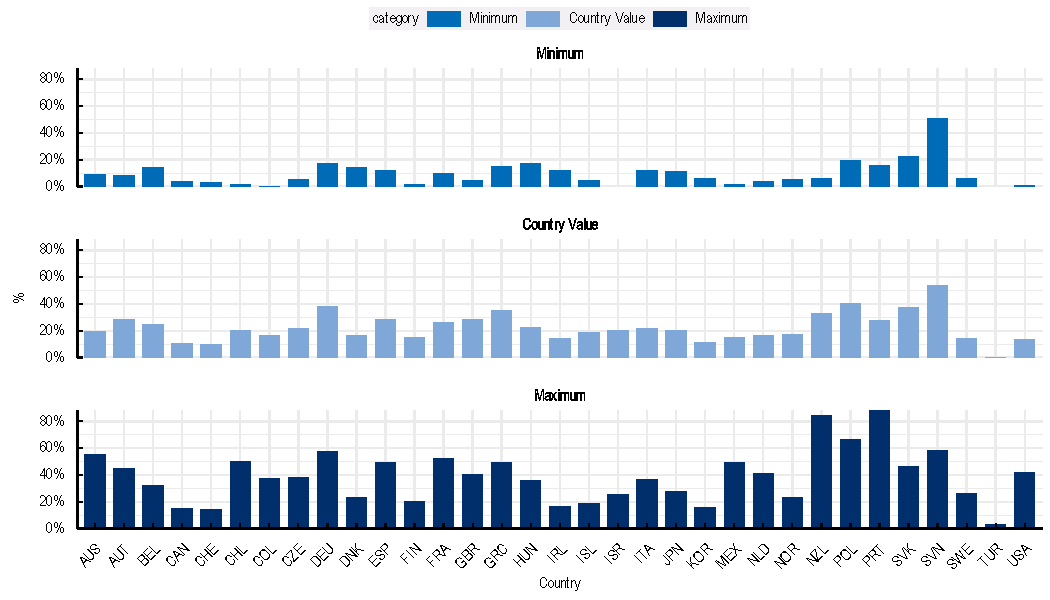
\includegraphics{reference_files/figure-latex/bar_final-1.pdf}

\hypertarget{basic-graph}{%
\subsubsection{Basic graph}\label{basic-graph}}

You can use fonts such as Arial Narrow within \texttt{ggplot2}. This
package allows that with a dedicated function. The first thing to do is
load in the libraries and data, as below:

\begin{Shaded}
\begin{Highlighting}[]
\FunctionTok{library}\NormalTok{(oecdplot)}
\FunctionTok{library}\NormalTok{(ggplot2)}
\FunctionTok{oecd\_load\_fonts}\NormalTok{()}
\end{Highlighting}
\end{Shaded}

In order to initialise a plot we tell ggplot that \texttt{pta} is our
data, and specify the variables on each axis. We then instruct ggplot to
render this as an bar plot by adding the \texttt{geom\_col} command. The
\texttt{position} argument separates the columns instead of the default
of displaying all the columns together.

\begin{Shaded}
\begin{Highlighting}[]
\NormalTok{p }\OtherTok{\textless{}{-}} \FunctionTok{ggplot}\NormalTok{(}\FunctionTok{aes}\NormalTok{(}\AttributeTok{x =}\NormalTok{ country, }\AttributeTok{y =}\NormalTok{ pct\_pta }\SpecialCharTok{/} \DecValTok{100}\NormalTok{, }\AttributeTok{fill =}\NormalTok{ category), }\AttributeTok{data =}\NormalTok{ pta) }\SpecialCharTok{+}
  \FunctionTok{geom\_col}\NormalTok{(}\AttributeTok{position =} \StringTok{"dodge2"}\NormalTok{)}
\NormalTok{p}
\end{Highlighting}
\end{Shaded}

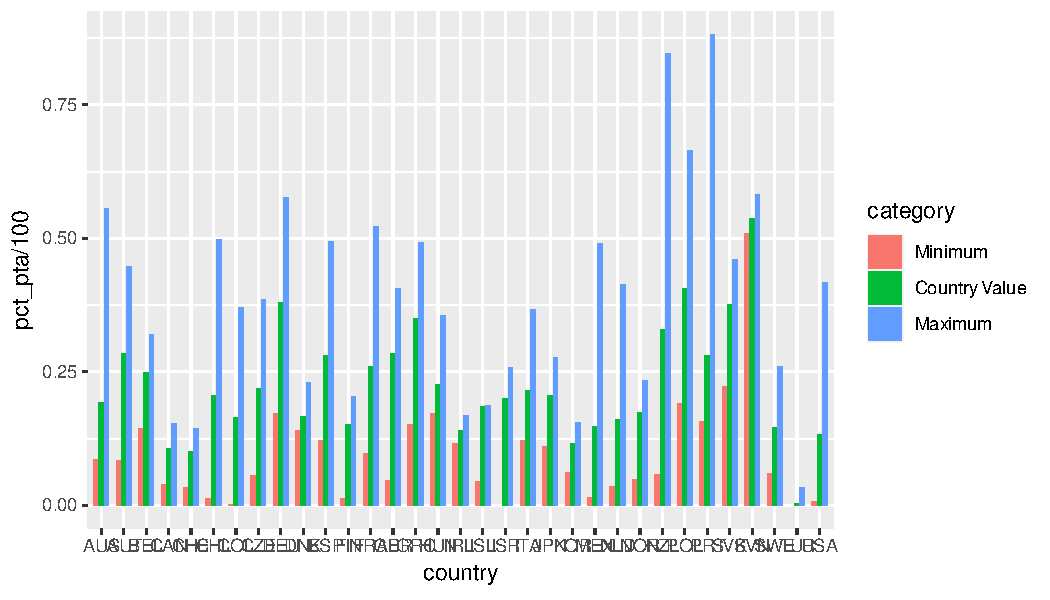
\includegraphics{reference_files/figure-latex/bar_1-1.pdf}

\hypertarget{adjusting-theme}{%
\subsubsection{Adjusting theme}\label{adjusting-theme}}

We can change the overall look of the graph using themes. We'll start
using a simple theme customisation by adding \texttt{theme\_oecd()}
after \texttt{ggplot()}.

\begin{Shaded}
\begin{Highlighting}[]
\NormalTok{p }\OtherTok{\textless{}{-}}\NormalTok{ p }\SpecialCharTok{+} 
  \FunctionTok{theme\_oecd}\NormalTok{()}
\NormalTok{p}
\end{Highlighting}
\end{Shaded}

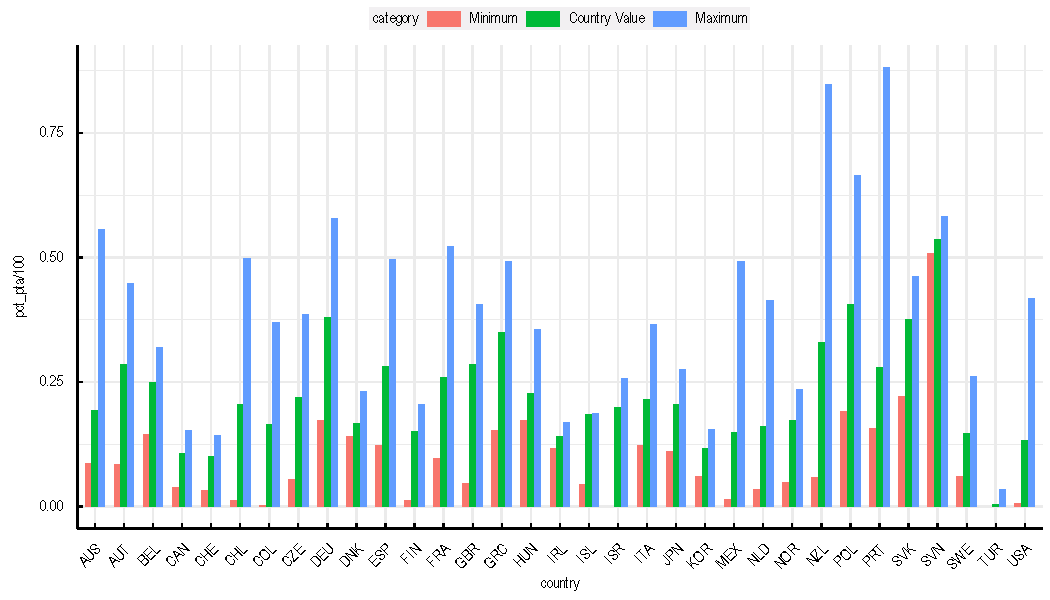
\includegraphics{reference_files/figure-latex/bar_2-1.pdf}

\hypertarget{adjusting-color-palette}{%
\subsubsection{Adjusting color palette}\label{adjusting-color-palette}}

To change the colours, we use the OECD scales. Note that you can
reference the specific colours you'd like to use with specific HEX
codes. You can also reference colours by name, with the full list of
colours recognised by R
\href{http://www.stat.columbia.edu/~tzheng/files/Rcolor.pdf}{here}. Here
we are using some arguments inside the scale function, in order to show
some of the personalization alternatives.

\begin{Shaded}
\begin{Highlighting}[]
\NormalTok{p }\OtherTok{\textless{}{-}}\NormalTok{ p }\SpecialCharTok{+}
  \FunctionTok{scale\_fill\_oecd\_d}\NormalTok{(}\AttributeTok{option =} \StringTok{"green"}\NormalTok{, }\AttributeTok{direction =} \SpecialCharTok{{-}}\DecValTok{1}\NormalTok{)}
\NormalTok{p}
\end{Highlighting}
\end{Shaded}

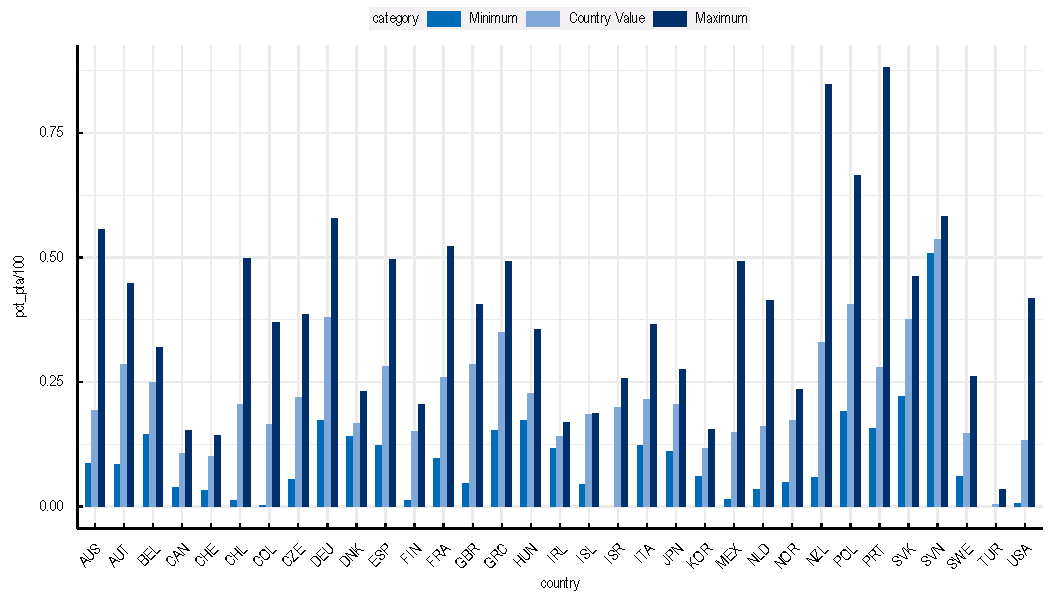
\includegraphics{reference_files/figure-latex/bar_3-1.pdf}

\hypertarget{adjusting-axis-scale}{%
\subsubsection{Adjusting axis scale}\label{adjusting-axis-scale}}

To change the scale to percentage, we use ggplot2 scale functions.

\begin{Shaded}
\begin{Highlighting}[]
\NormalTok{p }\OtherTok{\textless{}{-}}\NormalTok{ p }\SpecialCharTok{+}
  \FunctionTok{scale\_y\_continuous}\NormalTok{(}\AttributeTok{labels =}\NormalTok{ scales}\SpecialCharTok{::}\NormalTok{percent)}
\NormalTok{p}
\end{Highlighting}
\end{Shaded}

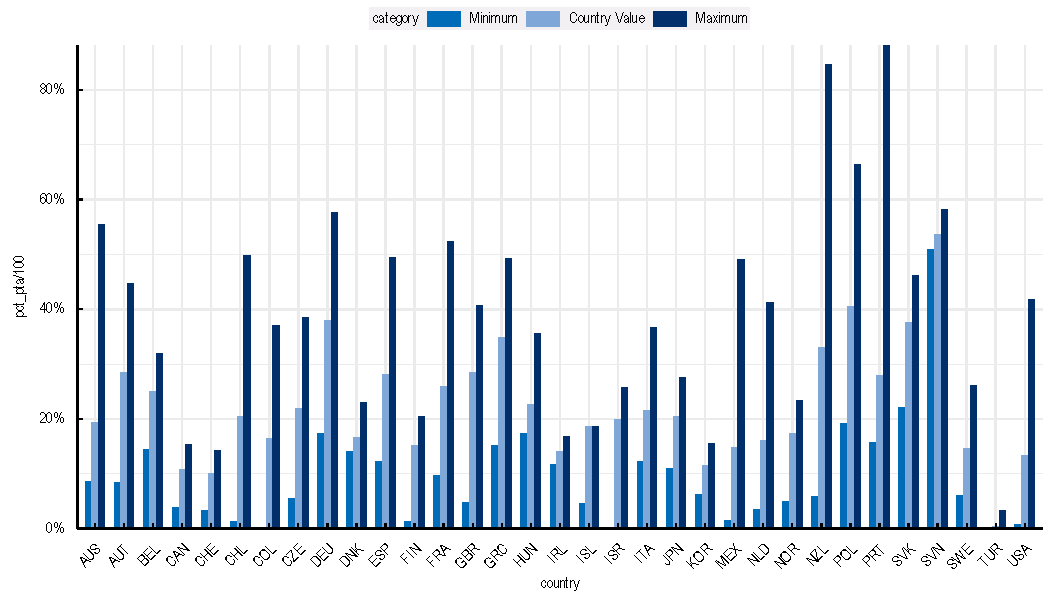
\includegraphics{reference_files/figure-latex/bar_4-1.pdf}

\hypertarget{facetting}{%
\subsubsection{Facetting}\label{facetting}}

In order to divide the resulting plot into a 3-in-1 plot, we use the
\texttt{facet\_wrap()} function. The \texttt{ncol} argument is used to
arrange the resulting plots in one column, instead of creating a three
columns layout in this case.

\begin{Shaded}
\begin{Highlighting}[]
\NormalTok{p }\OtherTok{\textless{}{-}}\NormalTok{ p }\SpecialCharTok{+}
  \FunctionTok{facet\_wrap}\NormalTok{(}\SpecialCharTok{\textasciitilde{}}\NormalTok{category, }\AttributeTok{ncol =} \DecValTok{1}\NormalTok{)}
\NormalTok{p}
\end{Highlighting}
\end{Shaded}

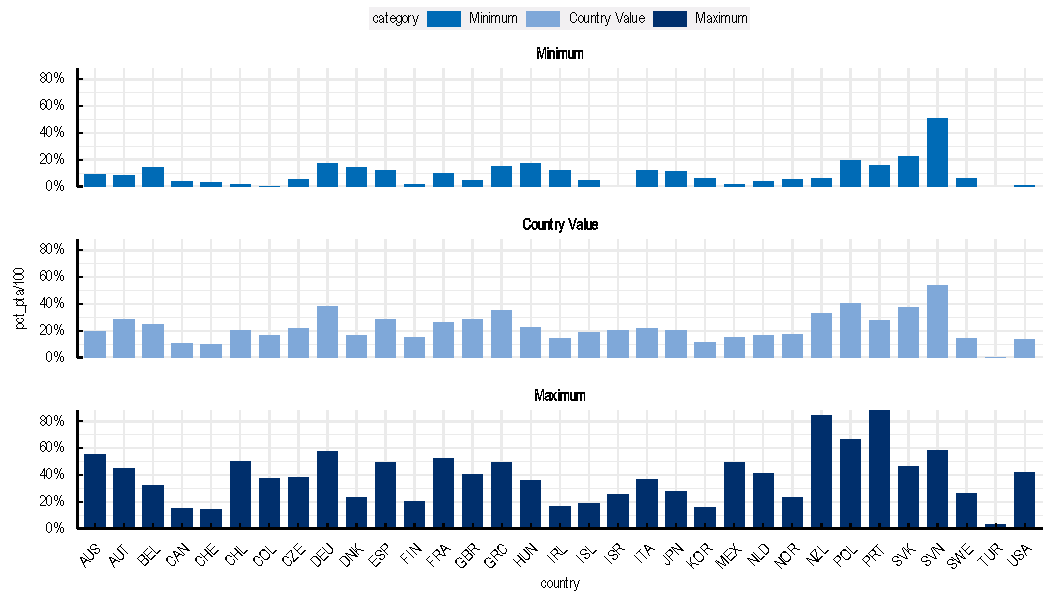
\includegraphics{reference_files/figure-latex/bar_5-1.pdf}

\hypertarget{adding-labels}{%
\subsubsection{Adding labels}\label{adding-labels}}

To obtain the plot from the start of this section, we use the
\texttt{labs()} function.

\begin{Shaded}
\begin{Highlighting}[]
\NormalTok{p }\OtherTok{\textless{}{-}}\NormalTok{ p }\SpecialCharTok{+}
  \FunctionTok{labs}\NormalTok{(}\AttributeTok{x =} \StringTok{"Country"}\NormalTok{, }\AttributeTok{y =} \StringTok{"\%"}\NormalTok{,}
       \AttributeTok{title =} \StringTok{"Protected terrestrial areas as a percentage of the total area"}\NormalTok{,}
       \AttributeTok{subtitle =} \StringTok{"Source: OECD Stat"}\NormalTok{)}
\NormalTok{p}
\end{Highlighting}
\end{Shaded}

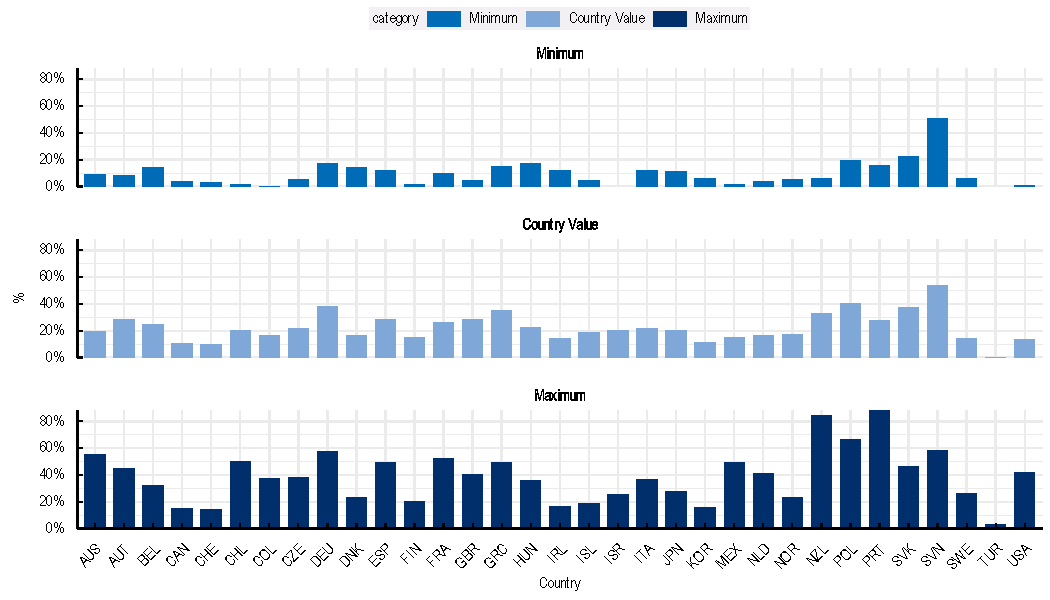
\includegraphics{reference_files/figure-latex/bar_6-1.pdf}

\hypertarget{scatterplots}{%
\subsection{Scatterplots}\label{scatterplots}}

We will work towards creating the scatterplot below. We will take you
from a basic bar plot and explain all the customisations we add to the
code step-by-step.

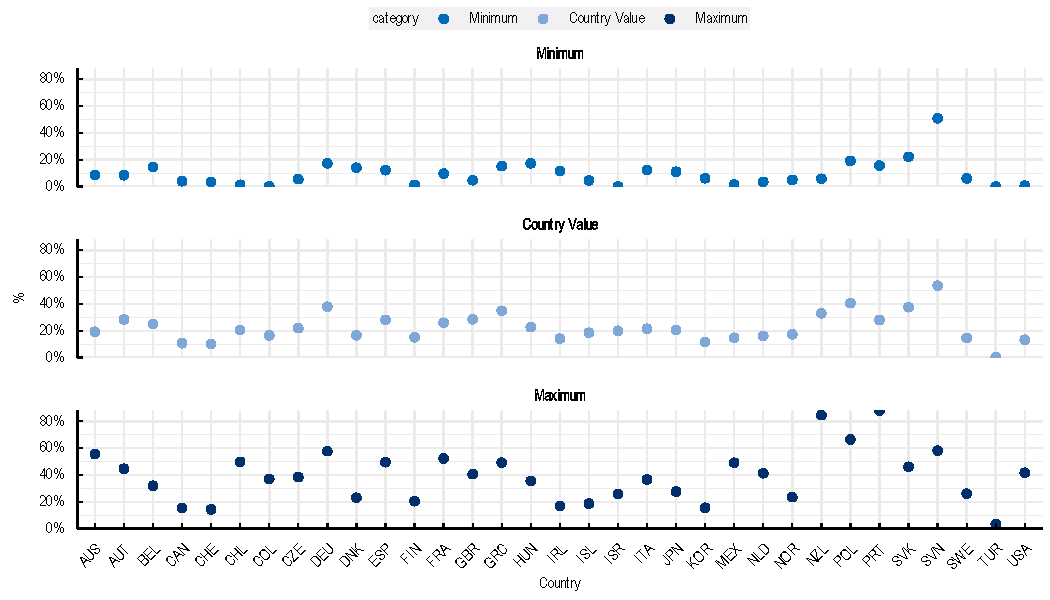
\includegraphics{reference_files/figure-latex/scatterplot_final-1.pdf}

\hypertarget{basic-graph-1}{%
\subsubsection{Basic graph}\label{basic-graph-1}}

You can use fonts such as Arial Narrow within \texttt{ggplot2}. This
package allows that with a dedicated function. The first thing to do is
load in the libraries and data, as below:

\begin{Shaded}
\begin{Highlighting}[]
\FunctionTok{library}\NormalTok{(oecdplot)}
\FunctionTok{library}\NormalTok{(ggplot2)}
\FunctionTok{oecd\_load\_fonts}\NormalTok{()}
\end{Highlighting}
\end{Shaded}

In order to initialise a plot we tell ggplot that \texttt{pta} is our
data, and specify the variables on each axis. We then instruct ggplot to
render this as an bar plot by adding the \texttt{geom\_point} command.

\begin{Shaded}
\begin{Highlighting}[]
\NormalTok{p }\OtherTok{\textless{}{-}} \FunctionTok{ggplot}\NormalTok{(}\FunctionTok{aes}\NormalTok{(}\AttributeTok{x =}\NormalTok{ country, }\AttributeTok{y =}\NormalTok{ pct\_pta }\SpecialCharTok{/} \DecValTok{100}\NormalTok{, }\AttributeTok{colour =}\NormalTok{ category), }\AttributeTok{data =}\NormalTok{ pta) }\SpecialCharTok{+}
  \FunctionTok{geom\_point}\NormalTok{()}
\NormalTok{p}
\end{Highlighting}
\end{Shaded}

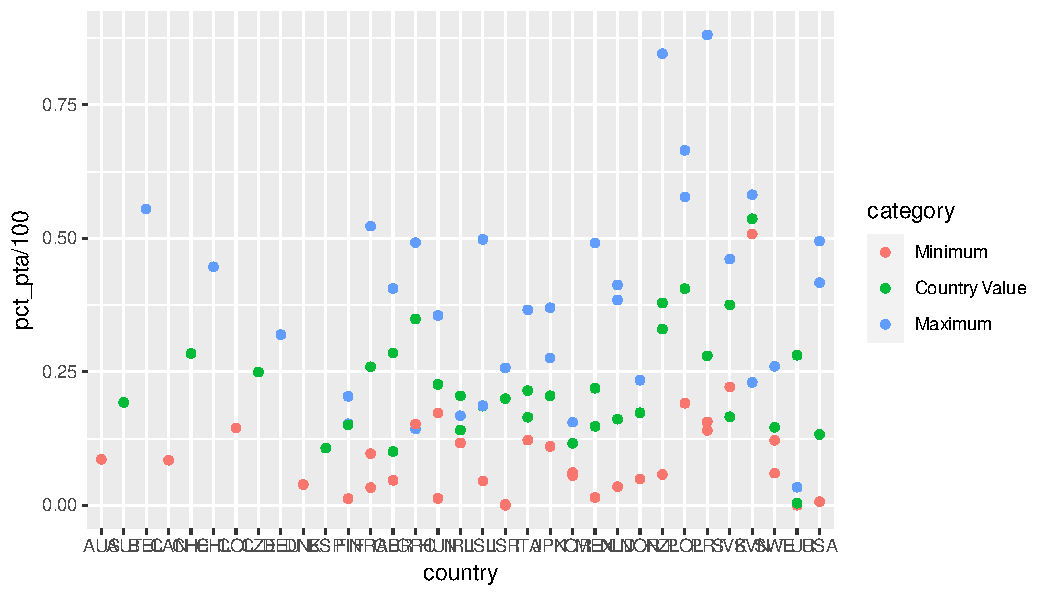
\includegraphics{reference_files/figure-latex/scatterplot_1-1.pdf}

\hypertarget{adjusting-theme-1}{%
\subsubsection{Adjusting theme}\label{adjusting-theme-1}}

We can change the overall look of the graph using themes. We'll start
using a simple theme customisation by adding \texttt{theme\_oecd()}
after \texttt{ggplot()}.

\begin{Shaded}
\begin{Highlighting}[]
\NormalTok{p }\OtherTok{\textless{}{-}}\NormalTok{ p }\SpecialCharTok{+} 
  \FunctionTok{theme\_oecd}\NormalTok{()}
\NormalTok{p}
\end{Highlighting}
\end{Shaded}

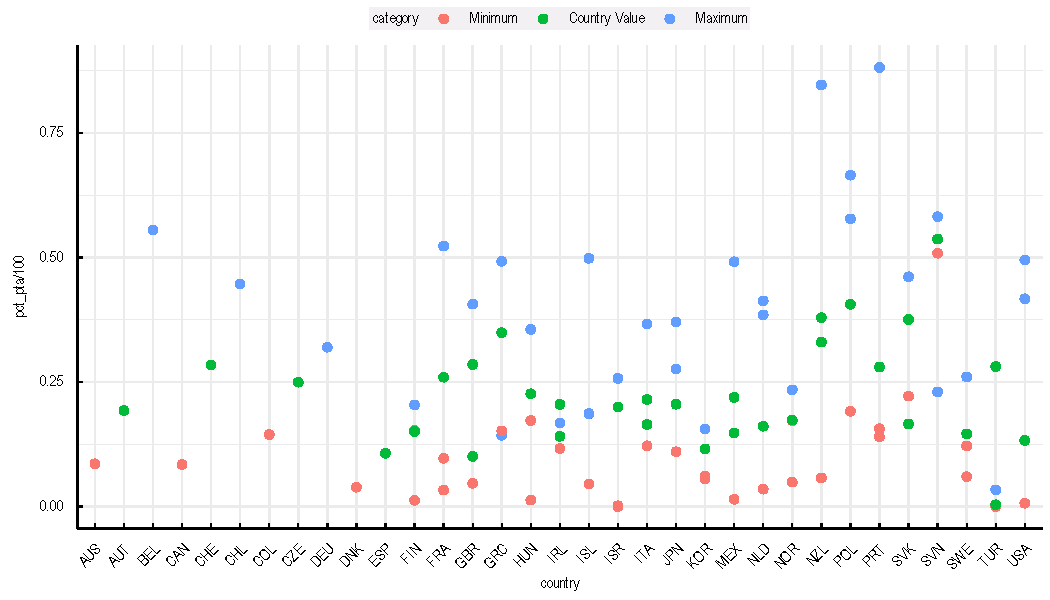
\includegraphics{reference_files/figure-latex/scatterplot_2-1.pdf}

\hypertarget{adjusting-color-palette-1}{%
\subsubsection{Adjusting color
palette}\label{adjusting-color-palette-1}}

To change the colours, we use the OECD scales. Note that you can
reference the specific colours you'd like to use with specific HEX
codes. You can also reference colours by name, with the full list of
colours recognised by R
\href{http://www.stat.columbia.edu/~tzheng/files/Rcolor.pdf}{here}. Here
we are using some arguments inside the scale function, in order to show
some of the personalization alternatives.

\begin{Shaded}
\begin{Highlighting}[]
\NormalTok{p }\OtherTok{\textless{}{-}}\NormalTok{ p }\SpecialCharTok{+}
  \FunctionTok{scale\_colour\_oecd\_d}\NormalTok{(}\AttributeTok{option =} \StringTok{"green"}\NormalTok{, }\AttributeTok{direction =} \SpecialCharTok{{-}}\DecValTok{1}\NormalTok{)}
\NormalTok{p}
\end{Highlighting}
\end{Shaded}

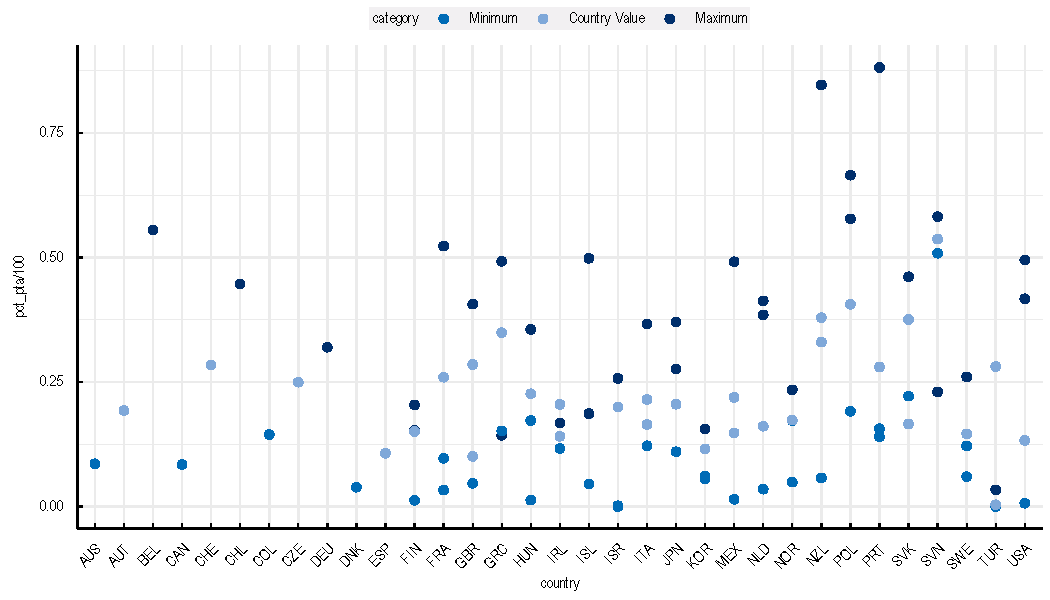
\includegraphics{reference_files/figure-latex/scatterplot_3-1.pdf}

\hypertarget{adjusting-axis-scale-1}{%
\subsubsection{Adjusting axis scale}\label{adjusting-axis-scale-1}}

To change the scale to percentage, we use ggplot2 scale functions.

\begin{Shaded}
\begin{Highlighting}[]
\NormalTok{p }\OtherTok{\textless{}{-}}\NormalTok{ p }\SpecialCharTok{+}
  \FunctionTok{scale\_y\_continuous}\NormalTok{(}\AttributeTok{labels =}\NormalTok{ scales}\SpecialCharTok{::}\NormalTok{percent)}
\NormalTok{p}
\end{Highlighting}
\end{Shaded}

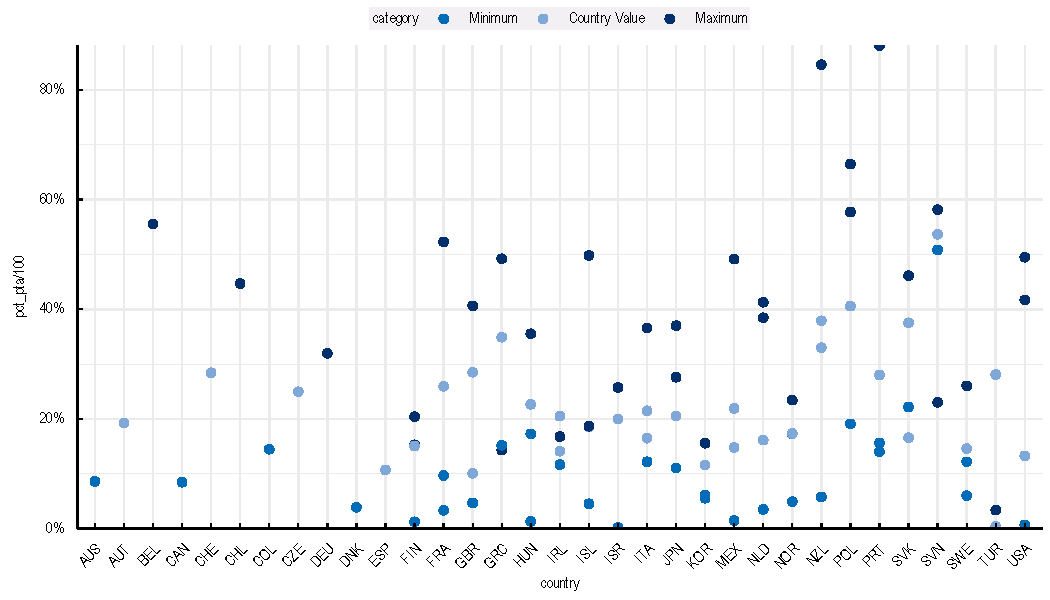
\includegraphics{reference_files/figure-latex/scatterplot_4-1.pdf}

\hypertarget{facetting-1}{%
\subsubsection{Facetting}\label{facetting-1}}

In order to divide the resulting plot into a 3-in-1 plot, we use the
\texttt{facet\_wrap()} function. The \texttt{ncol} argument is used to
arrange the resulting plots in one column, instead of creating a three
columns layout in this case.

\begin{Shaded}
\begin{Highlighting}[]
\NormalTok{p }\OtherTok{\textless{}{-}}\NormalTok{ p }\SpecialCharTok{+}
  \FunctionTok{facet\_wrap}\NormalTok{(}\SpecialCharTok{\textasciitilde{}}\NormalTok{category, }\AttributeTok{ncol =} \DecValTok{1}\NormalTok{)}
\NormalTok{p}
\end{Highlighting}
\end{Shaded}

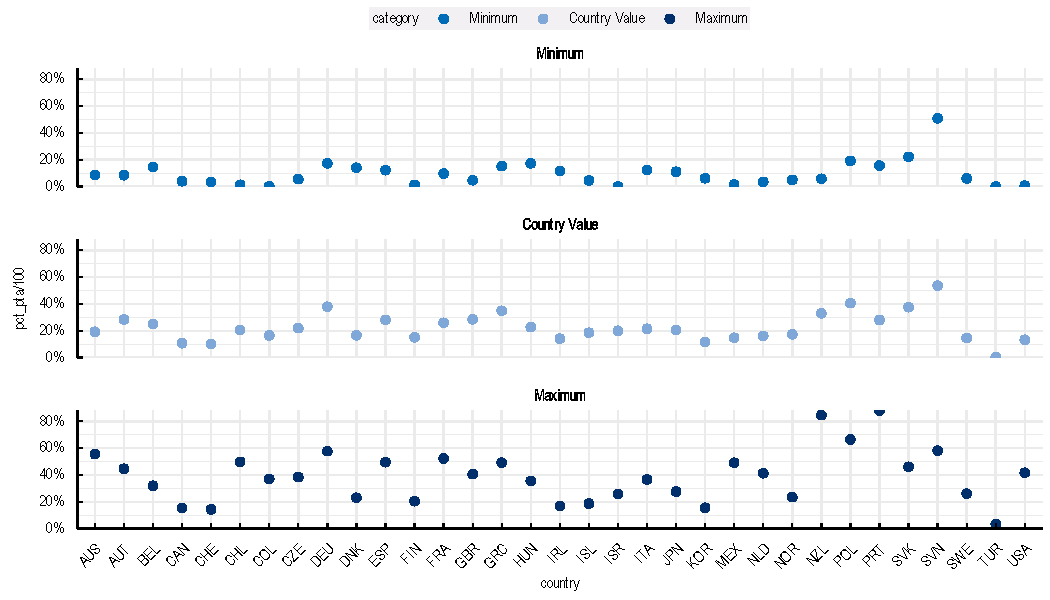
\includegraphics{reference_files/figure-latex/scatterplot_5-1.pdf}

\hypertarget{adding-labels-1}{%
\subsubsection{Adding labels}\label{adding-labels-1}}

To obtain the plot from the start of this section, we use the
\texttt{labs()} function.

\begin{Shaded}
\begin{Highlighting}[]
\NormalTok{p }\OtherTok{\textless{}{-}}\NormalTok{ p }\SpecialCharTok{+}
  \FunctionTok{labs}\NormalTok{(}\AttributeTok{x =} \StringTok{"Country"}\NormalTok{, }\AttributeTok{y =} \StringTok{"\%"}\NormalTok{,}
       \AttributeTok{title =} \StringTok{"Protected terrestrial areas as a percentage of the total area"}\NormalTok{,}
       \AttributeTok{subtitle =} \StringTok{"Source: OECD Stat"}\NormalTok{)}
\NormalTok{p}
\end{Highlighting}
\end{Shaded}

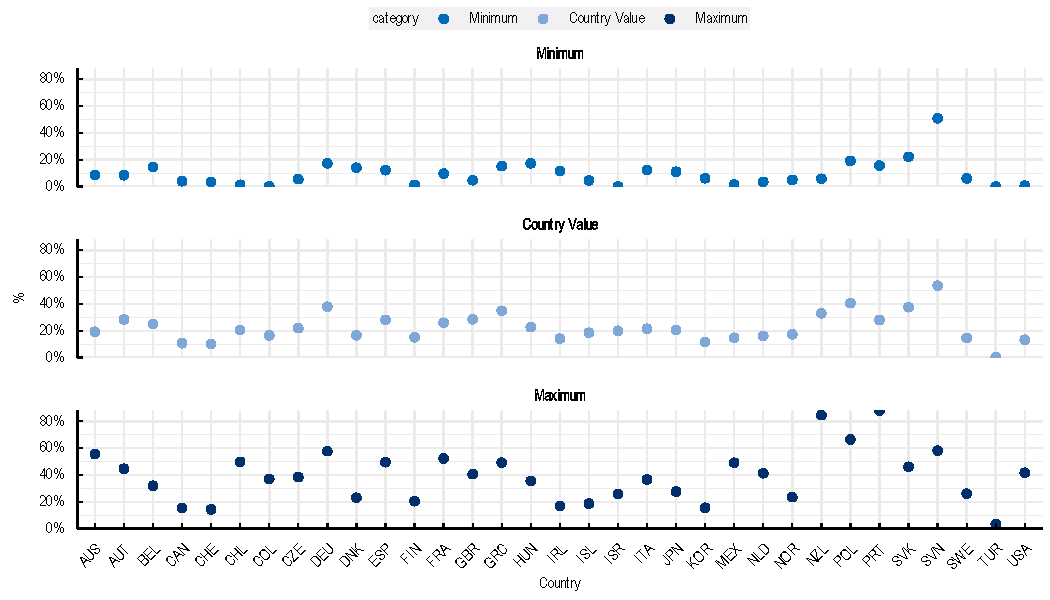
\includegraphics{reference_files/figure-latex/scatterplot_6-1.pdf}

\hypertarget{min-max-plots-scatterplot-line}{%
\subsection{Min-max plots (scatterplot +
line)}\label{min-max-plots-scatterplot-line}}

\emph{Warning:} This can be considered a very advanced plot.

We will work towards creating the bar plot below. We will take you from
a basic bar plot and explain all the customisations we add to the code
step-by-step.

\begin{verbatim}
## Warning: package 'dplyr' was built under R version 4.1.3
\end{verbatim}

\begin{verbatim}
## 
## Attaching package: 'dplyr'
\end{verbatim}

\begin{verbatim}
## The following objects are masked from 'package:stats':
## 
##     filter, lag
\end{verbatim}

\begin{verbatim}
## The following object is masked from 'package:testthat':
## 
##     matches
\end{verbatim}

\begin{verbatim}
## The following objects are masked from 'package:base':
## 
##     intersect, setdiff, setequal, union
\end{verbatim}

\begin{verbatim}
## Warning: package 'tidyr' was built under R version 4.1.3
\end{verbatim}

\begin{verbatim}
## 
## Attaching package: 'tidyr'
\end{verbatim}

\begin{verbatim}
## The following object is masked from 'package:testthat':
## 
##     matches
\end{verbatim}

\begin{verbatim}
## Joining, by = "country"
\end{verbatim}

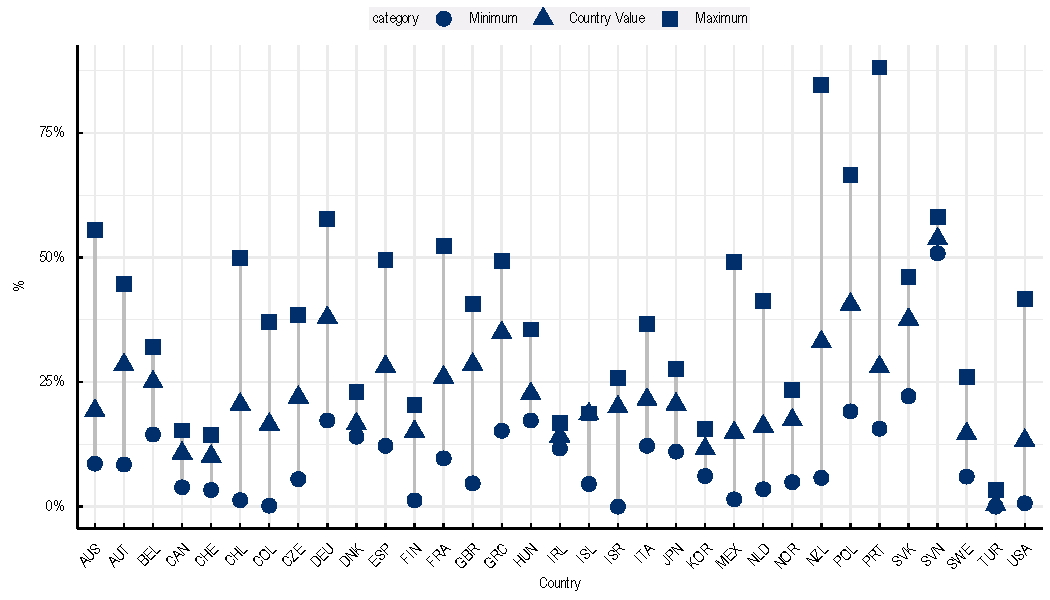
\includegraphics{reference_files/figure-latex/maxmin_final-1.pdf}

\hypertarget{reshaping-the-data}{%
\subsubsection{Reshaping the data}\label{reshaping-the-data}}

You can use fonts such as Arial Narrow within \texttt{ggplot2}. This
package allows that with a dedicated function. Because
\texttt{geom\_linerange()} requieres two columns, we must reshape the
data from the \texttt{oecdplot} package. The first thing to do is load
in the libraries and data, as below:

\begin{Shaded}
\begin{Highlighting}[]
\FunctionTok{library}\NormalTok{(oecdplot)}
\FunctionTok{library}\NormalTok{(ggplot2)}
\FunctionTok{library}\NormalTok{(dplyr)}
\FunctionTok{library}\NormalTok{(tidyr)}
\FunctionTok{oecd\_load\_fonts}\NormalTok{()}
\end{Highlighting}
\end{Shaded}

Now we can reshape the data to produce a max-min plot.

\begin{Shaded}
\begin{Highlighting}[]
\NormalTok{pta }\OtherTok{\textless{}{-}}\NormalTok{ pta }\SpecialCharTok{\%\textgreater{}\%} 
  \FunctionTok{mutate\_if}\NormalTok{(is.numeric, }\ControlFlowTok{function}\NormalTok{(x) x }\SpecialCharTok{/} \DecValTok{100}\NormalTok{)}

\NormalTok{pta2 }\OtherTok{\textless{}{-}}\NormalTok{ pta }\SpecialCharTok{\%\textgreater{}\%} 
  \FunctionTok{select}\NormalTok{(country, category, region) }\SpecialCharTok{\%\textgreater{}\%} 
  \FunctionTok{pivot\_wider}\NormalTok{(}\AttributeTok{values\_from =} \StringTok{"region"}\NormalTok{, }\AttributeTok{names\_from =} \StringTok{"category"}\NormalTok{) }\SpecialCharTok{\%\textgreater{}\%} 
  \FunctionTok{select}\NormalTok{(country, }\AttributeTok{reg\_min =}\NormalTok{ Minimum, }\AttributeTok{reg\_max =}\NormalTok{ Maximum) }\SpecialCharTok{\%\textgreater{}\%} 
  \FunctionTok{left\_join}\NormalTok{(}
\NormalTok{    pta }\SpecialCharTok{\%\textgreater{}\%} 
      \FunctionTok{select}\NormalTok{(country, category, pct\_pta) }\SpecialCharTok{\%\textgreater{}\%} 
      \FunctionTok{pivot\_wider}\NormalTok{(}\AttributeTok{values\_from =} \StringTok{"pct\_pta"}\NormalTok{, }\AttributeTok{names\_from =} \StringTok{"category"}\NormalTok{) }
\NormalTok{  ) }\SpecialCharTok{\%\textgreater{}\%} 
\NormalTok{  janitor}\SpecialCharTok{::}\FunctionTok{clean\_names}\NormalTok{()}
\end{Highlighting}
\end{Shaded}

\begin{verbatim}
## Joining, by = "country"
\end{verbatim}

\begin{Shaded}
\begin{Highlighting}[]
\NormalTok{pta2}
\end{Highlighting}
\end{Shaded}

\begin{verbatim}
## # A tibble: 33 x 6
##    country reg_min    reg_max                    minimum country_value maximum
##    <fct>   <fct>      <fct>                        <dbl>         <dbl>   <dbl>
##  1 NZL     Auckland   West Coast                 0.0577          0.330   0.846
##  2 PRT     Centro     Algarve                    0.156           0.280   0.881
##  3 CHL     Coquimbo   Aysén                      0.013           0.205   0.498
##  4 MEX     Guerrero   Baja California Sur        0.0147          0.148   0.491
##  5 POL     Lodzkie    Swietokrzyskie             0.191           0.406   0.665
##  6 AUS     Queensland Canberra Region (ACT)      0.0861          0.193   0.555
##  7 FRA     Brittany   Provence-Alpes-Côte d’Azur 0.0968          0.259   0.523
##  8 USA     Kansas     Alaska                     0.00680         0.133   0.417
##  9 DEU     Berlin     North Rhine-Westphalia     0.173           0.379   0.577
## 10 NLD     Groningen  Flevoland                  0.035           0.161   0.413
## # ... with 23 more rows
\end{verbatim}

\hypertarget{basic-graph-2}{%
\subsubsection{Basic graph}\label{basic-graph-2}}

In order to initialise a plot we tell ggplot that \texttt{pta2} is our
data, and specify the variables on each axis. We then instruct ggplot to
render this as an double plot by adding the \texttt{geom\_linerange()}
and \texttt{geom\_point()} functions. The shape specification here adds
visual aid.

\begin{Shaded}
\begin{Highlighting}[]
\NormalTok{p }\OtherTok{\textless{}{-}} \FunctionTok{ggplot}\NormalTok{() }\SpecialCharTok{+}
  \FunctionTok{geom\_linerange}\NormalTok{(}\AttributeTok{data =}\NormalTok{ pta2, }\FunctionTok{aes}\NormalTok{(}\AttributeTok{x =}\NormalTok{ country, }\AttributeTok{ymax =}\NormalTok{ maximum, }\AttributeTok{ymin =}\NormalTok{ minimum)) }\SpecialCharTok{+}
  \FunctionTok{geom\_point}\NormalTok{(}\AttributeTok{data =}\NormalTok{ pta, }
             \FunctionTok{aes}\NormalTok{(}\AttributeTok{x =}\NormalTok{ country, }\AttributeTok{y =}\NormalTok{ pct\_pta, }\AttributeTok{shape =}\NormalTok{ category), }
             \AttributeTok{colour =} \FunctionTok{oecd\_clrs}\NormalTok{()[}\DecValTok{1}\NormalTok{], }\AttributeTok{size =} \DecValTok{3}\NormalTok{)}

\NormalTok{p}
\end{Highlighting}
\end{Shaded}

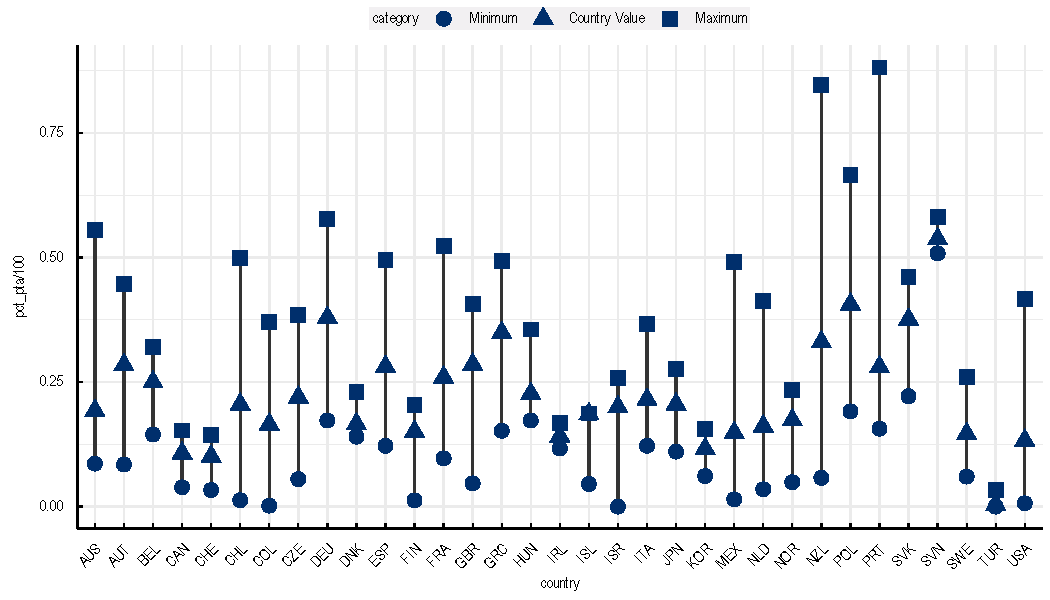
\includegraphics{reference_files/figure-latex/maxmin_2-1.pdf}

\hypertarget{adjusting-theme-2}{%
\subsubsection{Adjusting theme}\label{adjusting-theme-2}}

We can change the overall look of the graph using themes. We'll start
using a simple theme customisation by adding \texttt{theme\_oecd()}
after \texttt{ggplot()}.

\begin{Shaded}
\begin{Highlighting}[]
\NormalTok{p }\OtherTok{\textless{}{-}}\NormalTok{ p }\SpecialCharTok{+} 
  \FunctionTok{theme\_oecd}\NormalTok{(}\AttributeTok{base\_background =} \StringTok{"gray"}\NormalTok{)}
\NormalTok{p}
\end{Highlighting}
\end{Shaded}

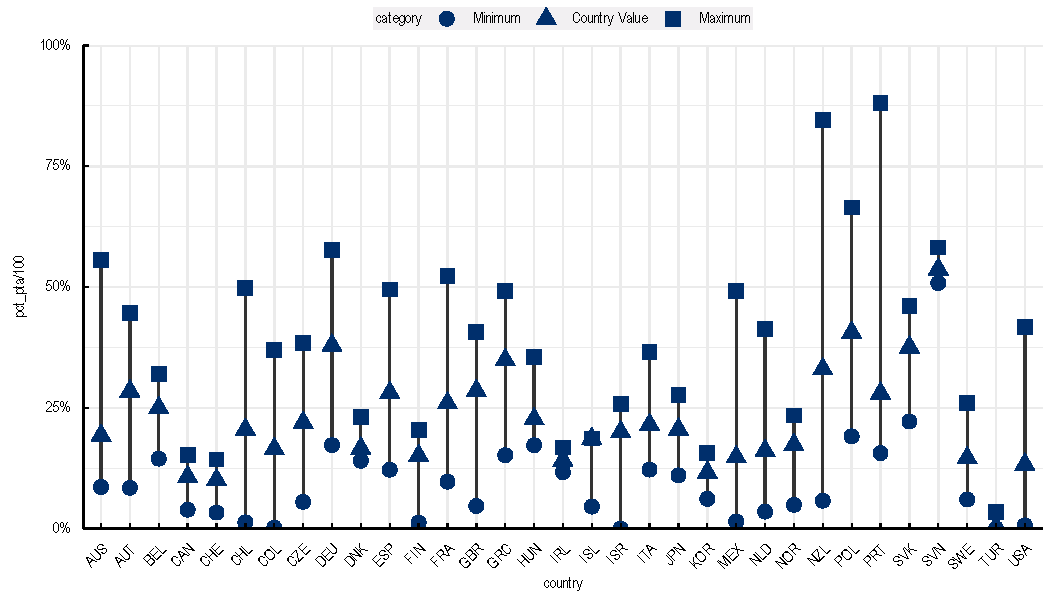
\includegraphics{reference_files/figure-latex/maxmin_3-1.pdf}

\hypertarget{adjusting-axis-scale-2}{%
\subsubsection{Adjusting axis scale}\label{adjusting-axis-scale-2}}

To change the scale to percentage, we use ggplot2 scale functions.

\begin{Shaded}
\begin{Highlighting}[]
\NormalTok{p }\OtherTok{\textless{}{-}}\NormalTok{ p }\SpecialCharTok{+}
  \FunctionTok{scale\_y\_continuous}\NormalTok{(}\AttributeTok{labels =}\NormalTok{ scales}\SpecialCharTok{::}\NormalTok{percent)}
\NormalTok{p}
\end{Highlighting}
\end{Shaded}

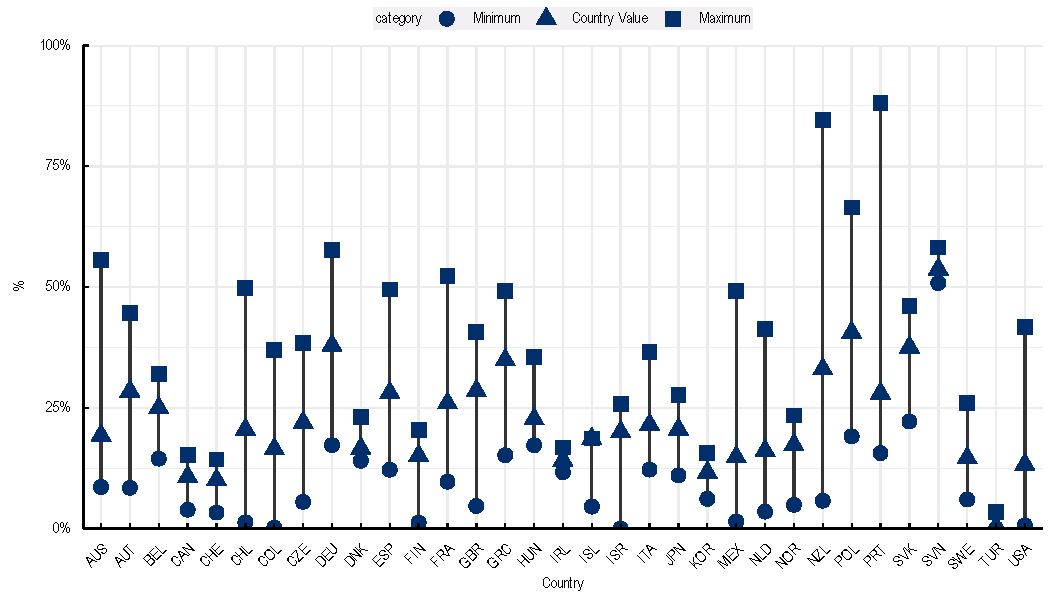
\includegraphics{reference_files/figure-latex/maxmin_4-1.pdf}

\hypertarget{adding-labels-2}{%
\subsubsection{Adding labels}\label{adding-labels-2}}

To obtain the plot from the start of this section, we use the
\texttt{labs()} function.

\begin{Shaded}
\begin{Highlighting}[]
\NormalTok{p }\OtherTok{\textless{}{-}}\NormalTok{ p }\SpecialCharTok{+}
  \FunctionTok{labs}\NormalTok{(}\AttributeTok{x =} \StringTok{""}\NormalTok{, }\AttributeTok{y =} \StringTok{""}\NormalTok{,}
       \AttributeTok{title =} \StringTok{"Protected terrestrial areas as a percentage of the total area"}\NormalTok{,}
       \AttributeTok{subtitle =} \StringTok{"Source: OECD Stat"}\NormalTok{)}
\NormalTok{p}
\end{Highlighting}
\end{Shaded}

\includegraphics{reference_files/figure-latex/maxmin_5-1.pdf}

\hypertarget{references}{%
\section{References}\label{references}}

Burchell, J., \& Vargas, M. (2019). \emph{The Hitchhiker's Guide to
Ggplot2}. Leanpub. URL: leanpub.com/ggplot-guide.

\end{document}
